% !TeX root = ../note.tex
\section{Моделирование предметной области}\label{sec:domain}

В разделе сформулированы функциональные требования для проектирования программного продукта.

\subsection{Описание сервисов программного продукта}\label{sec:domain:service}

% \subsubsection{} Сервис матчинга\label{sec:domain:service:matching}
\textbf{Сервис матчинга}

Основная задача биржи — проводить сделки между ордерами приходящими на биржу. В самом общем виде процесс происходит в следующем виде: пользователь выставляет свой ордер на покупку или продажу валюты, и начинается процесс матчинга, который может быть как быстрым, так и затянуться на часы ожидания. Пользователь биржи может выставлять разные типы ордеров с разными объёмами валюты для торгов. В зависимости от типа ордера и размера суммы ордера могут использоваться разные алгоритмы обработки ордера. В данном сервисе было решено реализовывать один тип ордера — отложенный лимитный ордер.

Лимитный ордер — это заявка на покупку или продажу определённого количества актива по указанной цене или лучше~\cite{limit_order}.

Лимитный ордер на покупку (buy limit) – это заявка на покупку по указанной цене или ниже (т.к. покупателю выгодно, чтобы цена была как можно меньше). Ордер buy limit выставляется по цене, которая ниже текущей рыночной. Трейдер использует этот ордер, когда надеется, что цена будет сначала падать, но потом, достигнув заданного уровня, развернётся и начнёт расти (т.е. он рассчитывает на отскок вверх от уровня поддержки, рис.~\ref{fig:orders_type}).

Лимитный ордер на продажу (sell limit) – это заявка на продажу по указанной цене или выше (т.к. продавцу выгодно, чтобы цена была как можно больше). Ордер sell limit выставляется по цене, которая выше текущей рыночной. Трейдер использует этот ордер, когда надеется, что цена будет сначала расти, но потом, достигнув заданного уровня, развернётся и начнёт падать (т.е. он рассчитывает на отскок вниз от уровня сопротивления, рис.~\ref{fig:orders_type}).

\begin{figure}[ht]
    \centering
    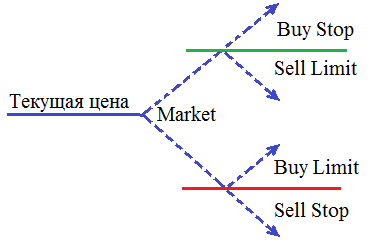
\includegraphics[scale=0.7]{orders.png}
    \caption{Цена исполнения ордеров различного типа относительно текущей цены}\label{fig:orders_type}
\end{figure}

Сервис хранит необходимую информацию, необходимую для обработки ордера, в оперативной памяти с целью обеспечения более быстрого доступа. Информация об ордерах и проведённых сделках хранится в соответствующих базах данных. Все главные модули должны работать в разных потоках. Также для обеспечения быстрой работы должна использоваться буферизация и пакетная запись в базу. Сервис и связанные с ним модули должны обеспечивать отказоустойчивость.

В функционал сервиса должны быть включены следующие модули:
\begin{itemize}
    \item логирование;
    \item интерфейс командной строки;
    \item конфигурация;
    \item восстановление данных;
    \item события UI.
\end{itemize}

% \begin{itemize}
    % \item логирование (п.~\ref{sec:domain:func:log});
    % \item интерфейс командной строки (п.~\ref{sec:domain:func:cli});
    % \item конфигурация (п.~\ref{sec:domain:func:config});
    % \item восстановление данных (п.~\ref{sec:domain:func:restore});
    % \item события UI (п.~\ref{sec:domain:func:events_ui}).
% \end{itemize}

% \subsubsection{} Сервис балансов\label{sec:domain:service:balance}
\textbf{Сервис балансов}

Все запросы, вызывающие изменение баланса, обрабатываются сервисом балансов (balance service). Получение информации о балансах происходит с помощью управляющих запросов. Из-за высокой нагрузки на этот модуль одному типу валюты должен соответствовать один сервис. Так же сервис балансов может шардироваться.

Данный сервис возвращает события об изменении балансов. Сервис и связанные с ним модули должны обеспечивать отказоустойчивость. База данных сервиса должна хранить балансы каждого пользователя и в каждой валюте, при этом если у пользователя нулевой баланс в какой-то из валют, то это пустое значение не должно храниться в базе данных (в случае обнуления баланса, запись о нём также должна удаляться).

В функционал сервиса должны быть включены следующие модули:
\begin{itemize}
    \item логирование;
    \item интерфейс командной строки;
    \item конфигурация;
    \item события UI.
\end{itemize}

% \begin{itemize}
%     \item логирование (п.~\ref{sec:domain:func:log});
%     \item интерфейс командной строки (п.~\ref{sec:domain:func:cli});
%     \item конфигурация (п.~\ref{sec:domain:func:config});
%     \item события UI (п.~\ref{sec:domain:func:events_ui}).
% \end{itemize}

% \subsubsection{} Сервис авторизации\label{sec:domain:service:auth}
\textbf{Сервис авторизации}

Сервис отвечает за регистрацию и аутентификацию пользователя. Для реализации регистрации/аутентификации должен использоваться стандарт JWT. Сервис работает с моделью пользователя в базе данных.

В функционал сервиса должны быть включены следующие модули:
\begin{itemize}
    \item логирование;
    \item интерфейс командной строки;
    \item конфигурация;
    \item восстановление данных;
    \item удалённый вызов процедур.
\end{itemize}

\subsection{Описание функциональных модулей программного продукта}\label{sec:domain:func}

% \subsubsection{} Логирование\label{sec:domain:func:log}
\textbf{Логирование}

Логер имеет интерфейс, предоставляющий API логирования различного уровня. Список доступных уровней:

\begin{itemize}
    \item debug — информация для отладки приложения;
    \item information  — уровень ''общей`` информации, иными словами вывод общей информации о происходящих в системе событиях, таких как создание ордера, обновление баланса, регистрация пользователя и т.д.;
    \item warning  — предупреждения об неправильном поведении сервиса;
    \item error — ошибка, при которой возможно продолжить работу сервиса;
    \item critical  — критическая ошибка, завершающая работу программы.
\end{itemize}

Уровни идут по возрастанию значимости (следовательно, если выставлен уровень information, то логи уровня debug выводиться не должны).

Логер записывает логи уровня error и critical в файл, переданный в конфигурации или как аргумент командной строки. Данные в файл записываются в формате JSON. Так же логер выводит в поток вывода (stdout) логи заданного через конфиг уровня.

Каждая запись в логах должна выводить сообщения в виде \lstinline{caller=<caller\_file>}, где файл и строка, вызвавшие лог и \lstinline{func=<caller\_func>} — название функции, вызвавшей логирование.

Логер должен иметь реализацию на интерфейсе, с целью быстрой подмены своей внутренней библиотеки. Для реализации рекомендуется использовать библиотеку log15~\cite{log_lib}.

% \subsubsection{} Работа с базами данных\label{sec:domain:func:database}
\textbf{Работа с базами данных}

В проекте используются различные типы данных, которые может быть нецелесообразно хранить в одной и той же базе данных, поэтому предполагается разработка общего интерфейса для доступа к базам данным. Предложенный подход позволит использовать один и тот же код для записи разных типов данных в разные базы данных, при этом для замены базе необходимо будет лишь заменить реализацию интерфейса для конкретной базы данных, не переделывая при этом основной код сервиса.

Предлагаемый общий интерфейс:
\begin{itemize}
    \item connect — подключение к базе данных;
	\item getByID — получение объекта из базы данных по уникальному идентификатору;
	\item add — добавление одного объекта в базу;
	\item addMany — добавление множества объектов в базу;
	\item update — обновление/замена одного объекта в базу;
	\item updateMany — обновление/замена множества объектов в базу;
	\item remove — удаление одного объекта из базы;
	\item removeMany — удаления множества объектов из базы;
	\item ping — проверка подключения к базе данных;
	\item close — закрытие подключения к базе данных.
\end{itemize}

Базы данных должны поддерживать репликацию для дальнейшего масштабирования сервиса.

% \subsubsection{} Интерфейс командной строки\label{sec:domain:func:cli}
\textbf{Интерфейс командной строки}

В сервисах должен быть реализован интерфейс командной сроки для запуска с различными параметрами. Параметры должны соответствовать стандарту интерфейса от GNU~\cite{gnu_cli}, то есть содержать аргументы в короткой форме (\lstinline{-h}), так и в полной (\lstinline{--version}). Опции должны включать в себя настройку всех необходимых для сервиса адресов, строк подключения к БД, названий файлов, очередей и каналов. Для обработки аргументов командной строки необходимо использовать какую-либо встроенную или качественно протестированную внешнюю библиотеку.

% \subsubsection{} Конфигурация
\textbf{Конфигурация}

Конфигурационный файл должен повторять все опции, используемые в сервисе из командной строки (кроме опции задающей сам конфигурационный файл). Формат файла — YAML. Для обработки параметров конфигурации необходимо использовать какую-либо встроенную или качественно протестированную внешнюю библиотеку. Желательно использовать библиотеку, которая может работать с параметрами командной строки.

% \subsubsection{} Восстановление данных
\textbf{Восстановление данных}

Сервисы, которые хранят данные в оперативной памяти (например ордеры в сервисе матчинге), должны иметь функционал для восстановления данных в память. Таким образом после аварийного или запланированного отключения сервиса, он сможет восстановить свою работу без потери данных.

% \subsubsection{} Сериализация
\textbf{Сериализация}

Сервисы должны использовать одинаковый вид сериализации для обмена данными в одинаковом формате. Сериализация и десериализация может быть как встроенной, так и производиться силами сторонней библиотеки.

% \subsubsection{} События UI
\textbf{События UI}

Данный дипломный проект создаётся с расчётом на своё дальнейшее развитие с добавление front-end части, поэтому на этапе проектирования необходимо предусмотреть механизм отправки событий, прослушивая которые можно обновлять элементы пользовательского интерфейса.

Примеры событий:
\begin{itemize}
    \item создание ордера;
    \item обновление ордера;
    \item удаление ордера;
    \item проведение сделки;
    \item внутренние ошибки сервиса.
\end{itemize}

% \subsubsection{} Очередь сообщений
\textbf{Очередь сообщений}

Для обмена данными между сервисами необходима очередь сообщений, гарантирующая доставку сообщений и целостность данных. Для сервиса матчинга требуется реализация отправки сообщений с ордерами. В свою очередь на баланс сервисе требуется реализация слушателя сообщений с ордерами.

% \subsubsection{} Удалённый вызов процедур
\textbf{Удалённый вызов процедур}

Модуль работы с RPC требуется для управления учётной записью пользователя на authority сервисе, т.е. для проведения операций регистрации и аутентификации.

\subsection{Описание моделей данных}\label{sec:domain:models}

% \subsubsection{} Модель ордера
\textbf{Модель ордера}

\begin{itemize}
    \item ID — уникальный идентификатор ордера;
    \item user ID — идентификатор владельца ордера;
    \item value — объём, выставленный на покупку или продажу в ордере;
    \item price — цена за единицу валюты;
    \item purchase — булевое значение, выставлен ли ордер на продажу или на покупку.
\end{itemize}

% \subsubsection{} Модель сделки\label{sec:domain:models:trade}
\textbf{Модель сделки}

\begin{itemize}
    \item ID — уникальный идентификатор сделки;
    \item buy order ID — идентификатор ордера на покупку;
    \item sell order ID — идентификатор ордера на продажу;
    \item buy user ID — идентификатор пользователя, который покупает валюту;
    \item sell user ID — идентификатор пользователя, который продаёт валюту;
    \item value — сумма сделки;
    \item price — цена за единицу валюты;
    \item time — время совершения сделки (формат UNIX Timestamp).
\end{itemize}

% \subsubsection{} Модель баланса\label{sec:domain:models:balance}
\textbf{Модель баланса}

\begin{itemize}
    \item ID — уникальный идентификатор пользователя;
    \item amount — количество валюты, доступное для использования;
    \item frozen amount — количество валюты, занятое в ордерах в данный момент.
\end{itemize}

% \subsubsection{} Модель пользователя\label{sec:domain:models:user}
\textbf{Модель пользователя}

\begin{itemize}
    \item ID — уникальный идентификатор пользователя;
    \item login — уникальный логин пользователя для аутентификации;
    \item email — уникальный пользовательский почтовый ящик;
    \item password hash — значение хеш-функции от пароля пользователя и некоторого модификатора входа (salt);
    \item token ID — токен для авторизации пользователя.
\end{itemize}

\subsection{Описание нефункциональных требований к программному продукту}\label{sec:domain:nonfunc}

% \subsubsection{} Документация\label{sec:domain:nonfunc:doc}
\textbf{Документация}

Документация к проекта должна быть написана в формате doxygen~\cite{doxygen}. Формат подразумевает полное описание классов, интерфейсов, методов, полей и т.д. прямо в коде с использованием специальных тегов для разметки документации. Автоматическая генерация документации должна быть настроена в проекте вместе с компиляцией самого проекта.

Пример документирования кода в doxygen:

% TODO: set style for c++
\lstinputlisting[language=C++,caption=Пример документированного C++ кода]{appendix/doxygen.cpp}

% \subsubsection{} Тестирование
\textbf{Тестирование}

Тестирование проекта необходимо осуществить на двух уровнях: юнит-тестирование и интеграционное тестирование. Тесты должны компилироваться вместе с проектом. Юнит-тестирование необходимо провести только для механизма матчинга. Необходимо протестировать как матчинг ордеров один к одному, так матчинг одного ордера с несколькими другими. Интеграционные тесты должны покрывать весь процесс от создания ордеров, до получения событий о сделках.
